\documentclass[aspectratio=169, 11pt]{beamer}

\usetheme{Madrid}
\usecolortheme{dolphin}

\usepackage[utf8]{inputenc}
\usepackage[T1]{fontenc}
\usepackage[spanish]{babel}
\usepackage{graphicx}
\usepackage{pdfpages}
\usepackage{booktabs}
\usepackage{array}
\usepackage{ragged2e}
\usepackage{hyperref}
\usepackage{amsmath, amssymb}


\usepackage{graphicx}
\usepackage{amsmath}
\usepackage{booktabs}
\usepackage{amssymb} % <-- para \checkmark
\usepackage{ifthen}  % <-- para condicionales simples
\setbeamertemplate{navigation symbols}{}
\setlength{\parskip}{4pt}
\justifying

\title{Transmisión de la política monetaria y dinámica inflacionaria en Colombia}
\subtitle{Evidencia empírica mediante un VARX(2)}
\author{Santiago Tupaz \\ Moisés Quintero}
\date{Febrero 2026}

\begin{document}

% ============================================================================
% SLIDE 1: PORTADA
% ============================================================================
\begin{frame}[plain]
\titlepage
\end{frame}

% ============================================================================
% SLIDE 2: MOTIVACIÓN EMPÍRICA
% ============================================================================
\begin{frame}{Motivación Empírica}
\vspace{-0.5cm}
\centering
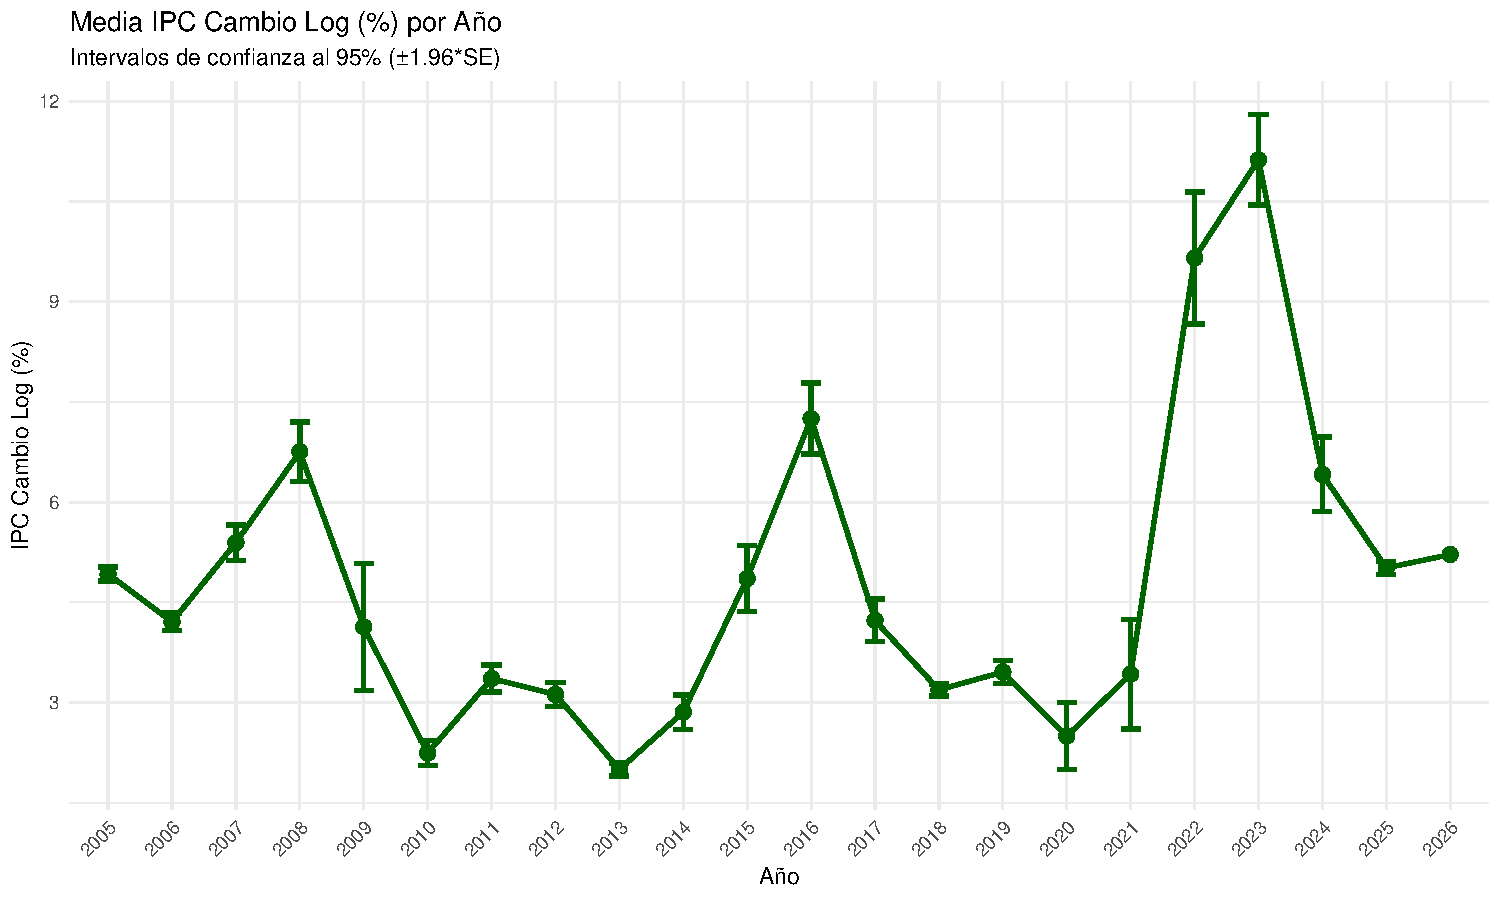
\includegraphics[width=0.95\textwidth, height=6.0cm]{../../outputs/EDA/05_mean_plot_IPC_log.pdf}
\vspace{0.1cm}
\small
\textit{Inflación en Colombia: ciclos 2008, 2020, 2021–2025. Política monetaria contractiva post-2022.}
\end{frame}

% ============================================================================
% SLIDE 3: PREGUNTA DE INVESTIGACIÓN Y CONTRIBUCIÓN
% ============================================================================
\begin{frame}{Pregunta de Investigación y Contribución}
\normalsize
\vspace{0.3cm}

\textbf{Pregunta central:}
\begin{itemize}
  \item ¿En qué medida choques monetarios (DTF) y financieros (TRM), junto con actividad (ISE), afectan la inflación anual en Colombia?
\end{itemize}

\vspace{0.3cm}
\textbf{Contribución:}
\begin{itemize}
  \item Estimación de \textbf{VARX(2) mensual} con bloque endógeno y control de shocks externos (inflación EE.UU., petróleo)
  \item Cuantificación de \textbf{dinámicas y rezagos} (IRF/FEVD) en contexto de economía abierta
  \item Validación predictiva (expanding window) vs benchmarks univariados
\end{itemize}
\end{frame}

% ============================================================================
% SLIDE 4: DATOS Y FUENTES
% ============================================================================
\begin{frame}{Datos y Fuentes}
\small
\vspace{0.2cm}

\begin{tabular}{lll}
\toprule
\textbf{Variable} & \textbf{Fuente} & \textbf{Frecuencia} \\
\midrule
Inflación Colombia (IPC) & DANE & Mensual \\
ISE desestacionalizado & DANE & Mensual \\
TRM (promedio) & Banco de la República & Mensual \\
DTF / CDT 90d & Banco de la República & Mensual \\
CPI-US (CPIAUCSL) & FRED & Mensual \\
Brent (DCOILBRENTEU) & FRED & Diario → Mensual \\
\bottomrule
\end{tabular}

\vspace{0.3cm}
\normalsize
\textbf{Período:} Enero 2006 — Noviembre 2025 (240 obs.). Estimación: 2006-01 a 2022-12. Validación OOS: 2023-01 a 2025-11.
\end{frame}

% ============================================================================
% SLIDE 5: EVIDENCIA DESCRIPTIVA — SERIES
% ============================================================================
\begin{frame}{Evidencia Descriptiva: Series Temporales}
\vspace{-0.5cm}
\centering
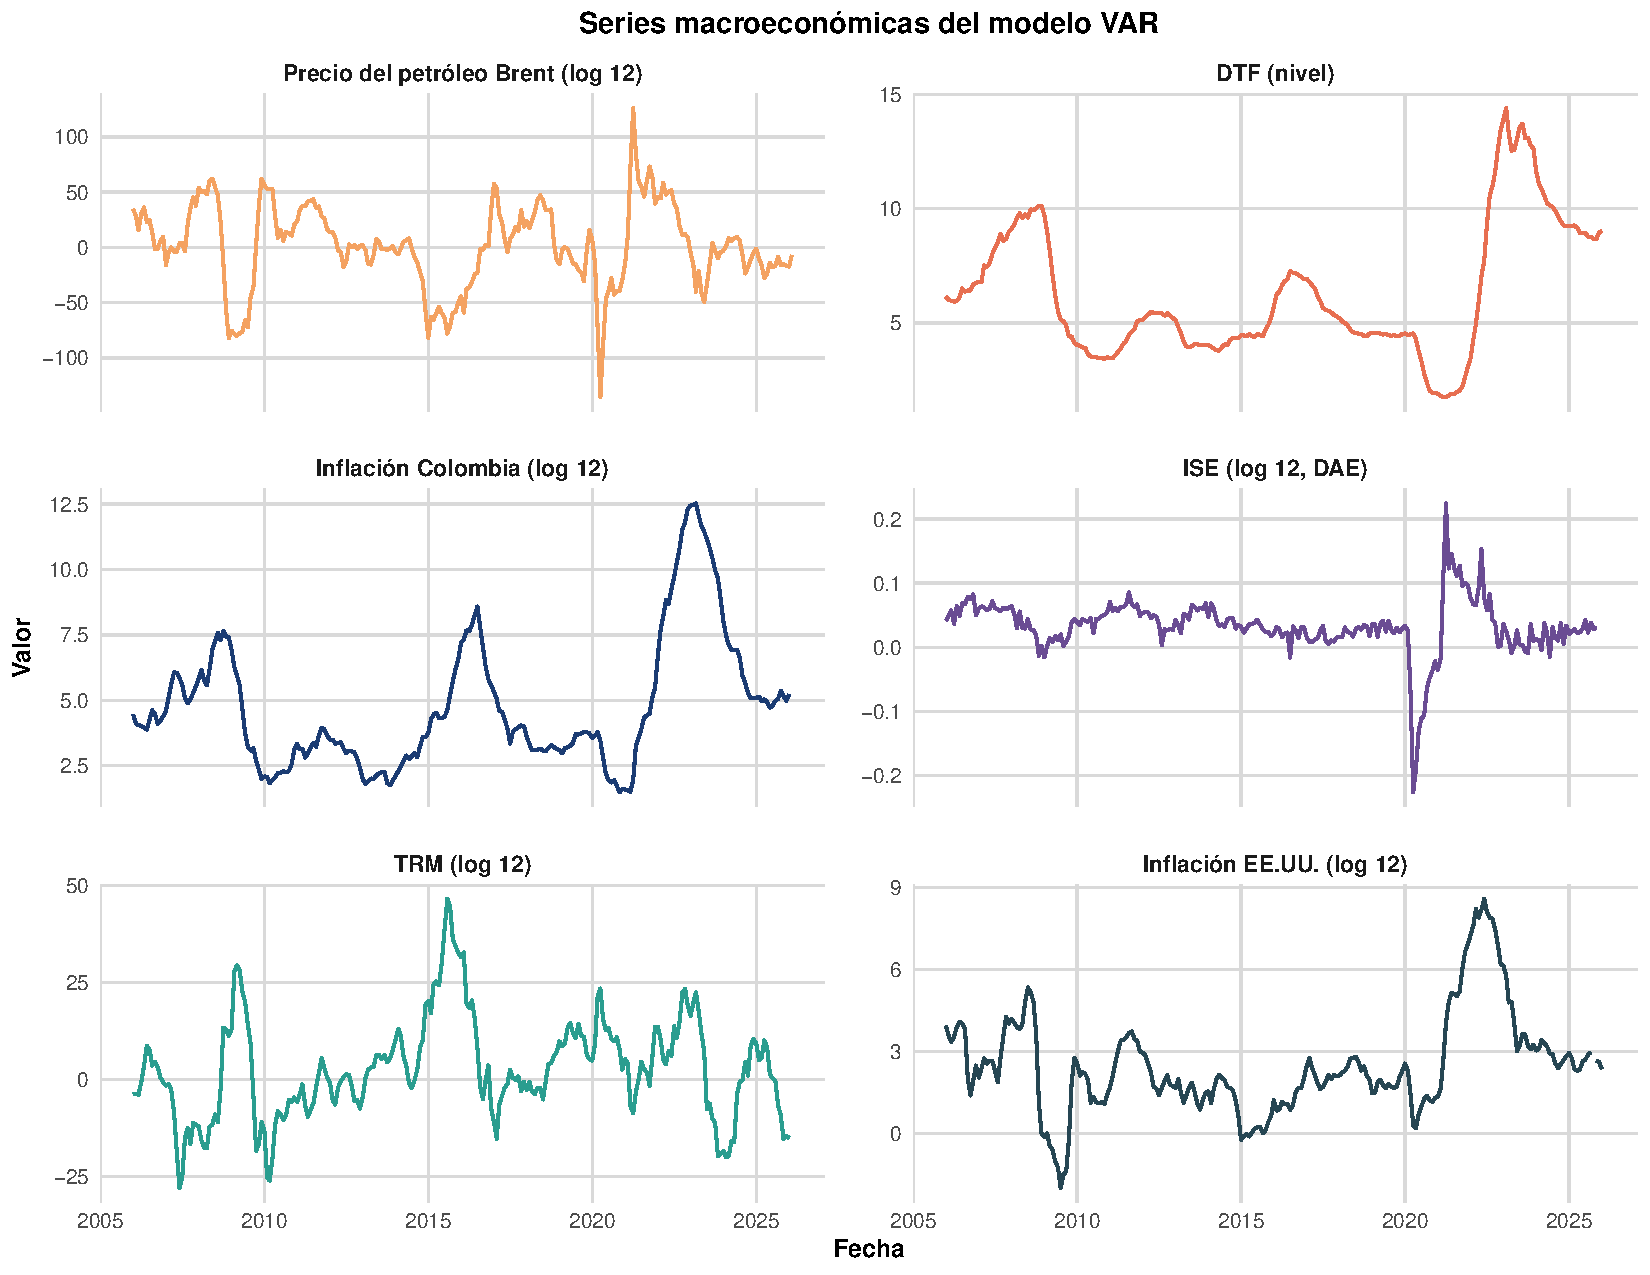
\includegraphics[width=0.95\textwidth, height=6.0cm]{../../outputs/VAR/01_series_macroeconomicas_VAR.pdf}
\vspace{0.1cm}
\small
Series mensuales: inflación, TRM, ISE, DTF. Variaciones conjuntas reflejan ciclos macro.
\end{frame}

% ============================================================================
% SLIDE 6: EVIDENCIA DESCRIPTIVA — DENSIDADES
% ============================================================================
\begin{frame}{Evidencia Descriptiva: Distribuciones}
\vspace{-0.5cm}
\centering
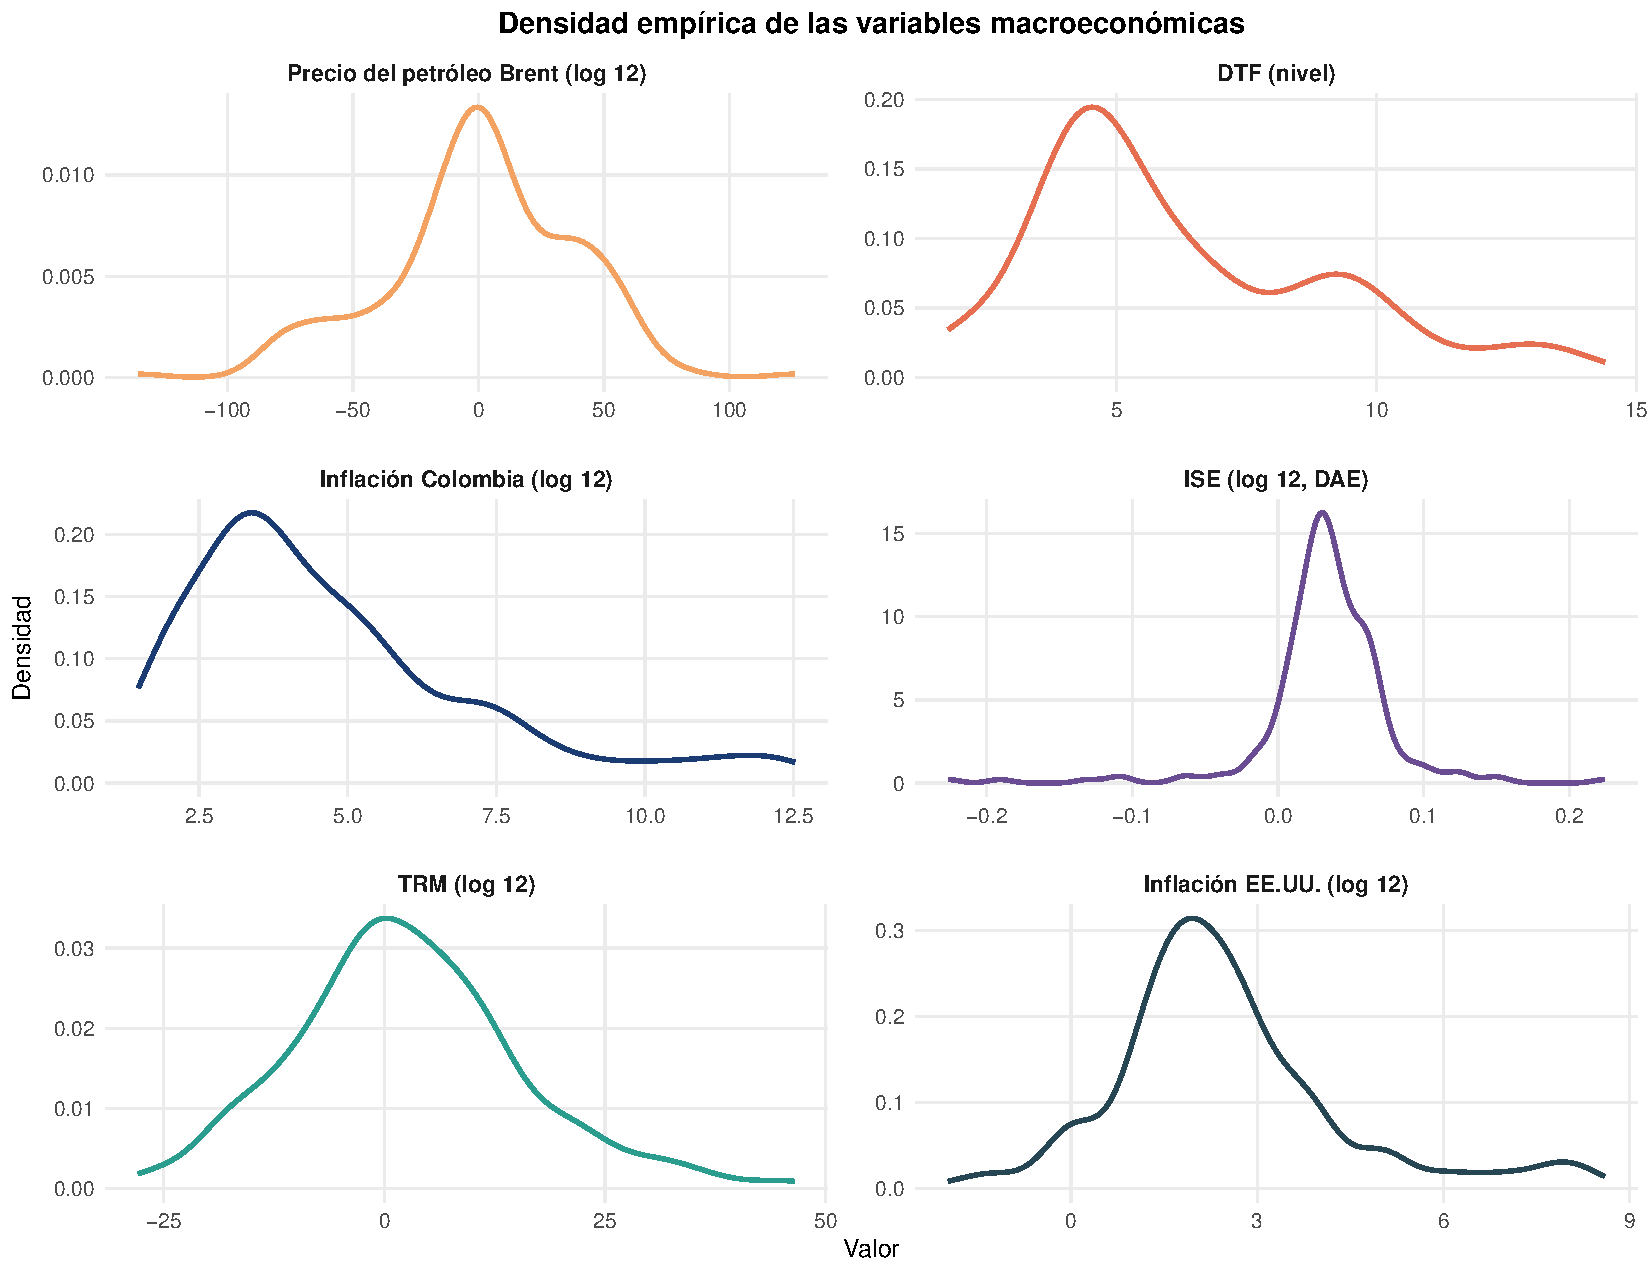
\includegraphics[width=0.95\textwidth, height=6.0cm]{../../outputs/VAR/03_densidades_6_variables.pdf}
\vspace{0.1cm}
\small
Densidades no-gaussianas: colas gruesas en variables financieras (TRM, DTF).
\end{frame}

% ============================================================================
% SLIDE 7: EVIDENCIA DESCRIPTIVA — CORRELACIONES (6 PÁGINAS)
% ============================================================================
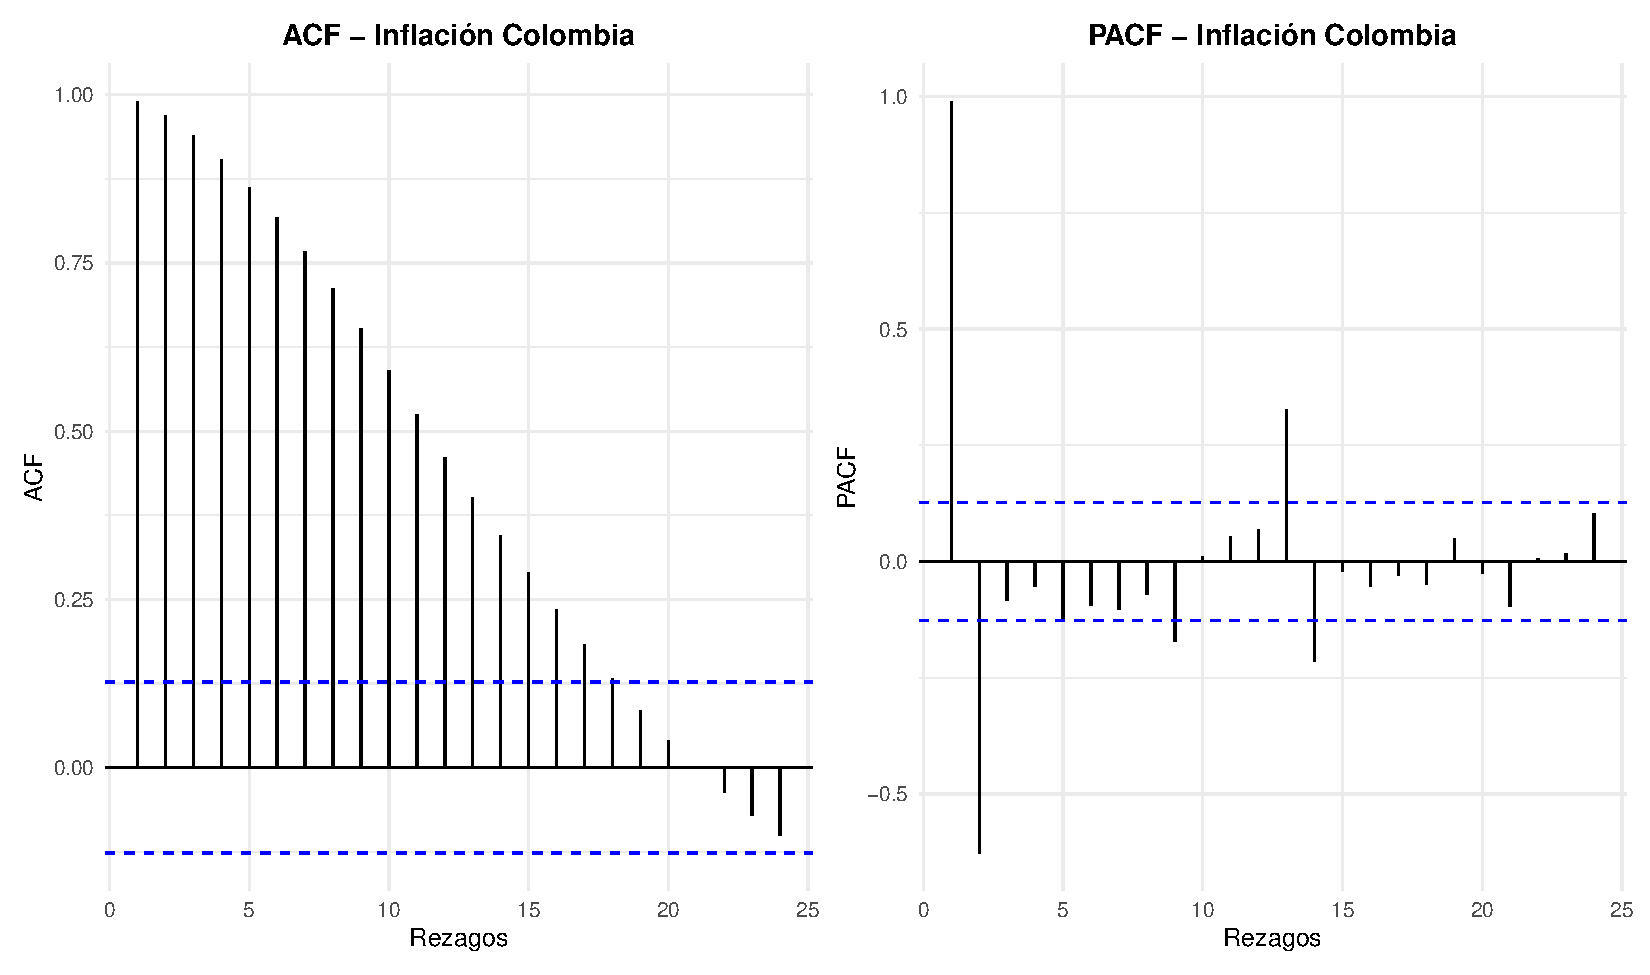
\includepdf[pages=1-6]{../../outputs/VAR/04_correlogramas_6_variables.pdf}

% ============================================================================
% SLIDE 8: TRANSFORMACIONES Y ESPECIFICACIÓN DE VARIABLES
% ============================================================================
\begin{frame}{Transformaciones y Especificación de Variables}
\normalsize
\vspace{0.2cm}

\textbf{Bloque endógeno (4 variables):}
\begin{align*}
\pi_t &= \Delta_{12}\log(\text{IPC}_t) \times 100 \quad \text{[variación anual IPC]} \\
\text{TRM}_t &= \Delta_{12}\log(\text{TRM}_t) \times 100 \quad \text{[depreciación anual]} \\
\text{ISE}_t &= \Delta_{12}\log(\text{ISE}_t) \times 100 \quad \text{[actividad anual]} \\
\text{DTF}_t &= \text{Nivel (pp)} \quad \text{[tasa nominal]}
\end{align*}

\textbf{Bloque exógeno (2 variables):}
\begin{align*}
\pi^{US}_t &= \Delta_{12}\log(\text{CPI-US}_t) \times 100 \quad \text{[inflación exterior]} \\
\text{Brent}_t &= \Delta_{12}\log(\text{Brent}_t) \times 100 \quad \text{[shock de oferta]}
\end{align*}

\small
\textit{Justificación:} $\Delta_{12}\log$ para estacionariedad relativa; DTF en nivel para interpretabilidad de postura monetaria.
\end{frame}

% ============================================================================
% SLIDE 9: ESTACIONARIEDAD CON QUIEBRE (ZIVOT–ANDREWS)
% ============================================================================
\begin{frame}[fragile]{Validación Econométrica: Raíz Unitaria}
\scriptsize
\begin{center}
\begin{tabular}{lrrrcp{3.0cm}}
\toprule
\textbf{Variable} & \textbf{PP} & \textbf{KPSS} & \textbf{ZA} & \textbf{Quiebre} & \textbf{Conclusión} \\
\midrule
Inflación & 0.695 & 0.010* & -3.54 & Oct-20 & Persistencia + quiebre \\
TRM & 0.045* & 0.071 & -3.93 & May-08 & Evidencia mixta \\
DTF & 0.807 & 0.011* & -4.94$^\dagger$ & Oct-20 & Persistencia (nivel) \\
ISE & 0.010* & 0.100 & -4.43 & Sep-19 & Estacionaria en tasas \\
Inflación US & 0.243 & 0.010* & -3.72 & Sep-19 & Persistencia nominal \\
Brent & 0.010* & 0.100 & -3.40 & Jul-19 & Estacionaria en tasas \\
\bottomrule
\end{tabular}
\end{center}

\vspace{0.2cm}
\tiny
\textit{Nota:} PP (H$_0$: raíz unitaria), KPSS (H$_0$: estacionaria). ZA con quiebre endógeno (modelo ``both''). * p$<$0.05. $\dagger$ Rechaza al 10\% pero no al 5\%.
\end{frame}

% ============================================================================
% SLIDE 10: ESPECIFICACIÓN VARX(2)
% ============================================================================
\begin{frame}{Especificación: VARX(2)}
\normalsize
\vspace{0.3cm}

\textbf{Forma reducida:}
\[
\mathbf{y}_t = \mathbf{c} + \mathbf{A}_1 \mathbf{y}_{t-1} + \mathbf{A}_2 \mathbf{y}_{t-2} + \mathbf{B} \mathbf{x}_t + \mathbf{u}_t
\]

\small
donde $\mathbf{y}_t = (\pi_t, \Delta_{12}\log(\text{TRM}_t), \Delta_{12}\log(\text{ISE}_t), \text{DTF}_t)'$ (endógenas, $4 \times 1$)

$\mathbf{x}_t = (\pi^{US}_t, \Delta_{12}\log(\text{Brent}_t))'$ (exógenas contemporáneas, $2 \times 1$)

\vspace{0.3cm}
\normalsize
\textbf{Selección:} $p = 2$ rezagos por AIC/HQ/SC/FPE.

\textbf{Identificación:} Orden Cholesky: $\pi_t \to \text{TRM}_t \to \text{ISE}_t \to \text{DTF}_t$ (económicamente justificado).

\textbf{Estimación:} OLS. Inferencia dinámica: bootstrap 95\% (2000 réplicas) para IRFs.
\end{frame}

% ============================================================================
% SLIDE 11: DIAGNÓSTICO RESIDUAL
% ============================================================================
\begin{frame}{Diagnóstico Residual Multivariado}
\small
\vspace{0.2cm}

\begin{tabular}{lcp{3cm}}
\toprule
\textbf{Prueba} & \textbf{p-value} & \textbf{Conclusión} \\
\midrule
Portmanteau (h=6) & $1.615 \times 10^{-8}$ & Rechaza $H_0$: autocorrelación presente \\
LM Breusch–Godfrey (h=6) & $8.924 \times 10^{-9}$ & Rechaza $H_0$: dependencia serial multivariada \\
ARCH multivariado (12) & $1.36 \times 10^{-10}$ & Rechaza $H_0$: heterocedasticidad condicional \\
Normalidad Jarque–Bera & $< 2.2 \times 10^{-16}$ & Rechaza $H_0$: colas gruesas, no-normalidad \\
\bottomrule
\end{tabular}

\vspace{0.3cm}
\normalsize
\textit{Consistente con colas gruesas y volatilidad condicionada en series macro-financieras mensuales. Decisión: mantener VARX(2); inferencia dinámica vía bootstrap no paramétrico (robusto a no-normalidad).}
\end{frame}

% ============================================================================
% SLIDE 12: RAÍCES Y ESTABILIDAD
% ============================================================================
\begin{frame}{Estabilidad del Sistema: Raíces Características}
\vspace{-0.5cm}
\centering
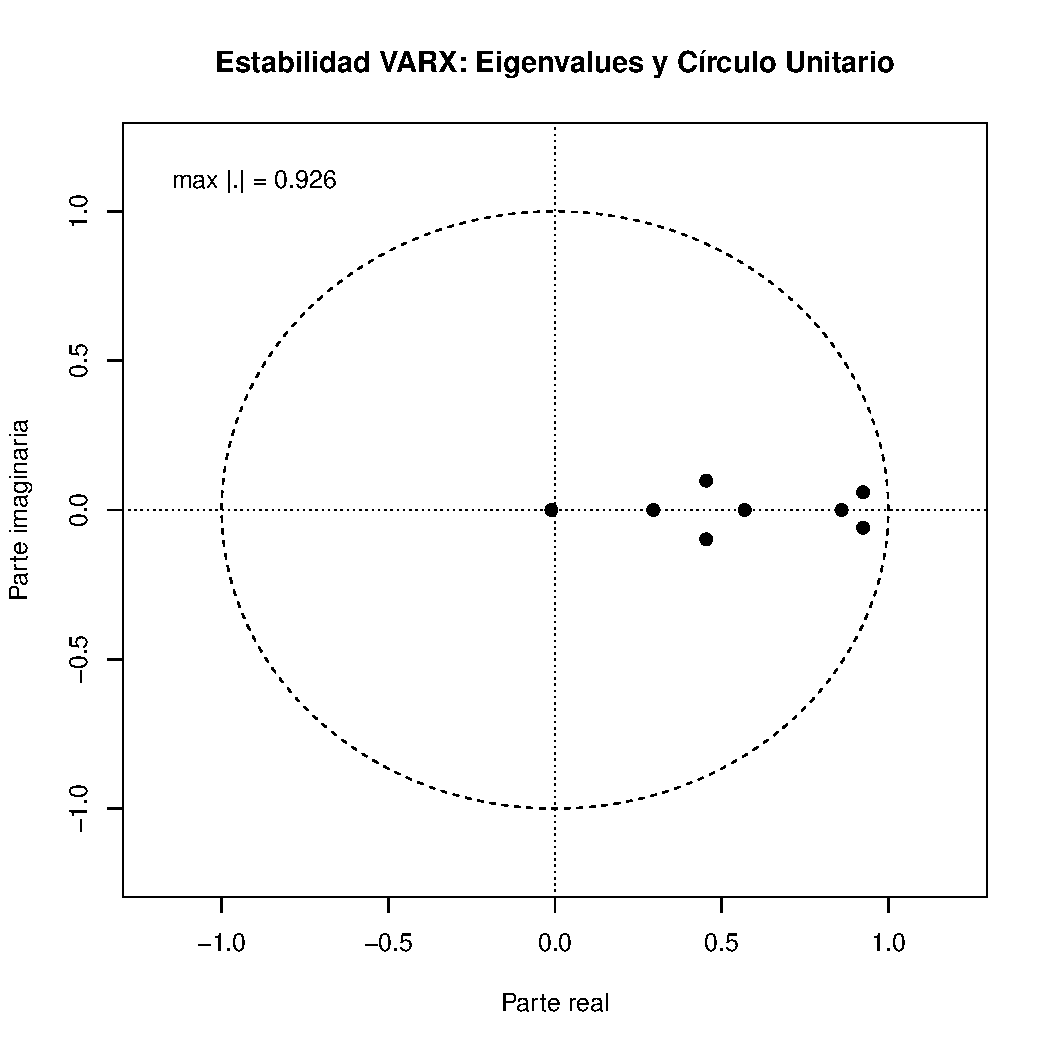
\includegraphics[width=0.95\textwidth, height=6.5cm]{../../outputs/VAR/05_raices_varx_circulo_unitario.pdf}
\vspace{0.1cm}
\small
Todas las raíces dentro del círculo unitario: $|\lambda_{\max}| \approx 0.926 < 1$. \textbf{Sistema dinámicamente estable.}
\end{frame}

% ============================================================================
% SLIDE 13: RESULTADOS DINÁMICOS — IRF (3 PÁGINAS)
% ============================================================================
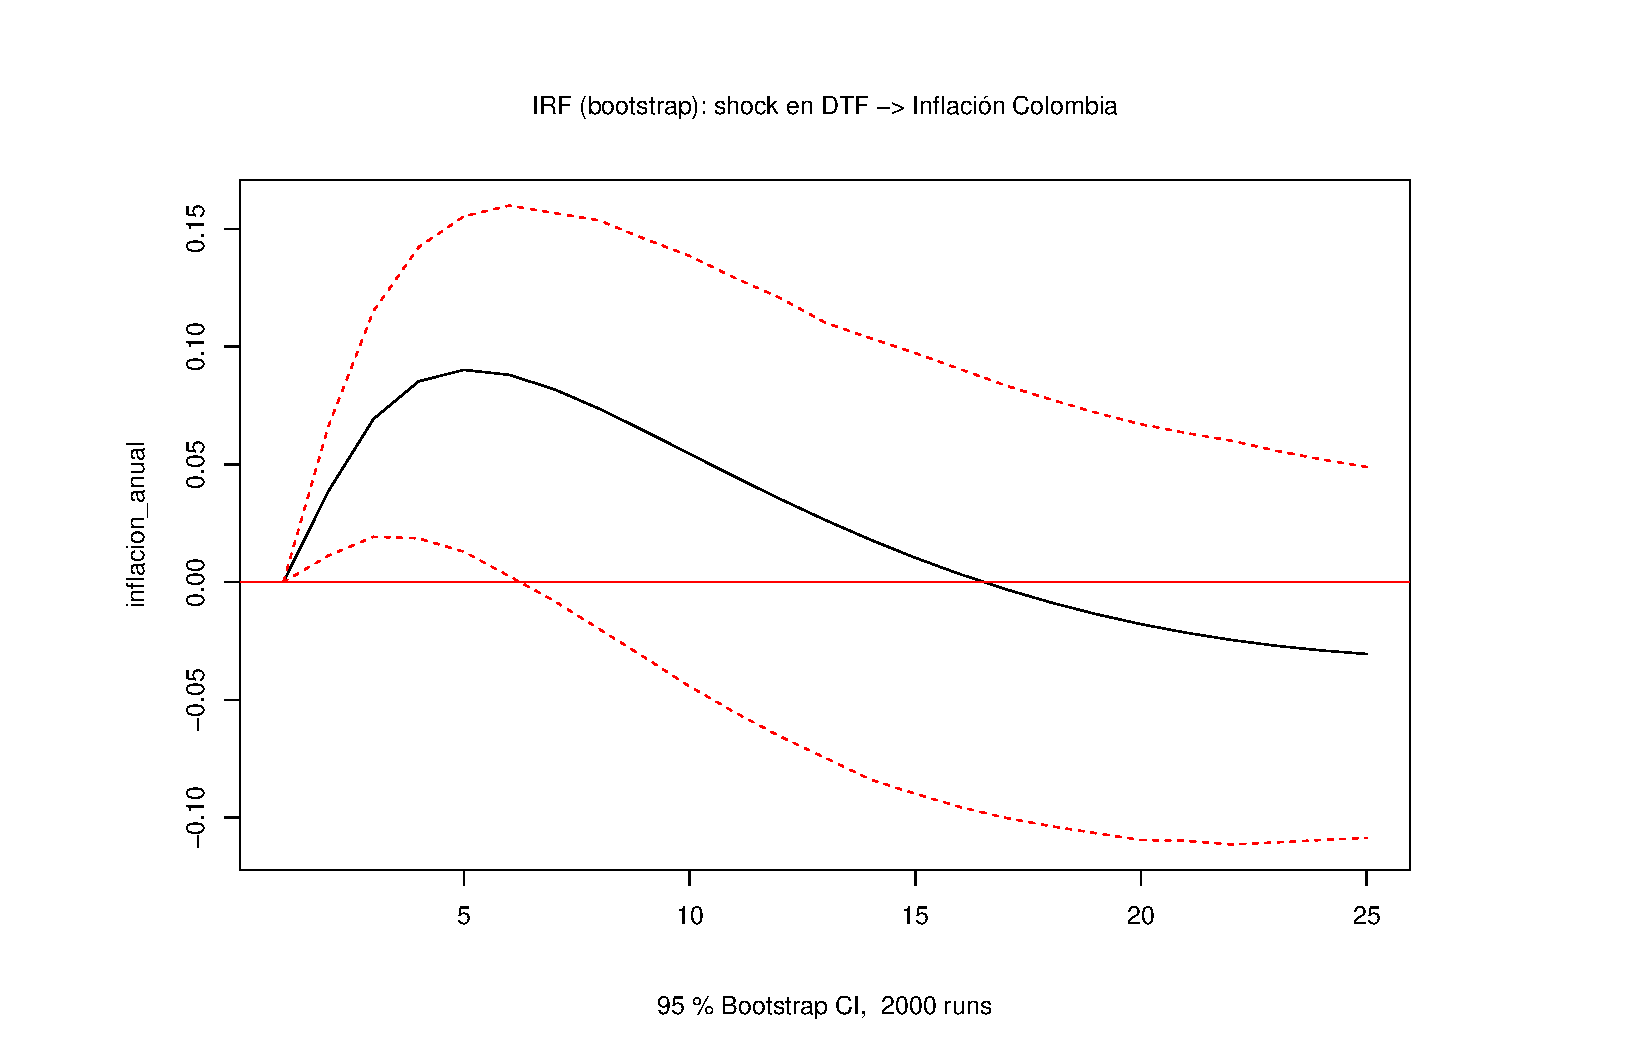
\includepdf[pages=1-3]{../../outputs/VAR/08_irf_bootstrap_inflacion.pdf}

% ============================================================================
% SLIDE 14: RESULTADOS DINÁMICOS — FEVD
% ============================================================================
\begin{frame}{Resultados Dinámicos: Descomposición de Varianza (FEVD)}
\small
\vspace{0.2cm}

\begin{tabular}{lccccc}
\toprule
\textbf{Horizonte} & \textbf{1m} & \textbf{3m} & \textbf{6m} & \textbf{12m} & \textbf{24m} \\
\midrule
\textbf{Shock a $\pi$ (propio)} & 100\% & 85\% & 62\% & 45\% & 34\% \\
\textbf{Shock a TRM} & 0\% & 9\% & 20\% & 31\% & 39\% \\
\textbf{Shock a ISE} & 0\% & 5\% & 15\% & 21\% & 25\% \\
\textbf{Shock a DTF} & 0\% & 1\% & 2\% & 2\% & 3\% \\
\bottomrule
\end{tabular}

\vspace{0.25cm}
\normalsize
\textbf{Lectura:}
\begin{itemize}
  \item Corto plazo (h $\leq$ 3m): persistencia inflacionaria domina.
  \item Mediano–largo (h $\geq$ 12m): canales cambiario (TRM) + real (ISE) = 60\% de varianza.
  \item Canal monetario (DTF) débil (~3\%): transmisión limitada.
\end{itemize}
\end{frame}

% ============================================================================
% SLIDE 15: VALIDACIÓN PREDICTIVA (EXPANDING WINDOW)
% ============================================================================
\begin{frame}{Validación Predictiva: Expanding Window OOS}
\small
\vspace{0.2cm}

\begin{tabular}{lcccc}
\toprule
\textbf{Horizonte} & \textbf{VARX RMSE} & \textbf{ARIMA RMSE} & \textbf{Naive RMSE} & \textbf{Ganancia VARX} \\
\midrule
$h = 1$ mes & 0.82 & 0.71 & 2.10 & $-15\%$ (ARIMA mejor) \\
$h = 3$ meses & 0.85 & 1.61 & 3.20 & \textbf{+47\%} vs ARIMA \\
$h = 6$ meses & 1.25 & 3.53 & 5.10 & \textbf{+65\%} vs ARIMA \\
$h = 12$ meses & 2.10 & 6.20 & 7.85 & \textbf{+66\%} vs ARIMA \\
\bottomrule
\end{tabular}

\vspace{0.2cm}
\normalsize
\textbf{Interpretación:} VARX supera univariados en horizontes mediano–largo (h $\geq$ 3m). Información macroeconómica (TRM, ISE, DTF) es valiosa para pronósticos operacionales. Corto plazo (h=1m): ARIMA competitivo.
\end{frame}

% ============================================================================
% SLIDE 16: PRONÓSTICO 2026
% ============================================================================
\begin{frame}{Pronóstico 2026: Escenario Base}
\vspace{-0.5cm}
\centering
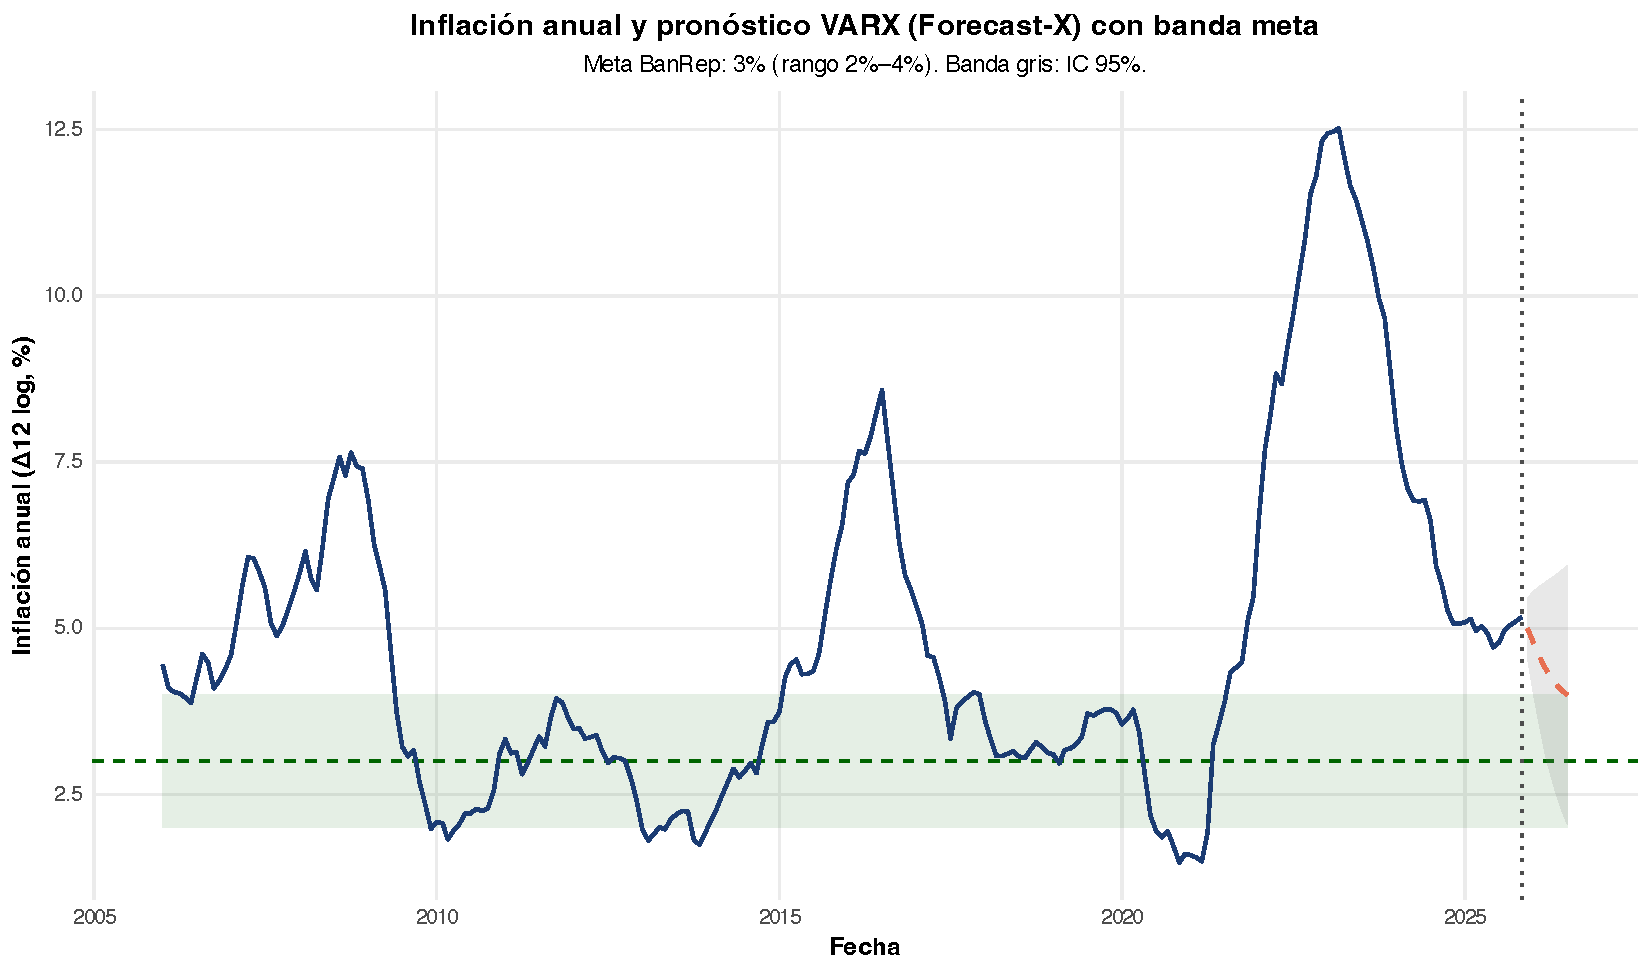
\includegraphics[width=0.95\textwidth, height=6.0cm]{../../outputs/VAR/09_forecast_inflacion_varx_banda_meta.pdf}
\vspace{0.1cm}
\small
Pronóstico condicionado (Forecast-X). Banda meta BanRep: 2\%–4\%. Línea meta: 3\%. Desinflación gradual compatible con objetivo.
\end{frame}

% ============================================================================
% SLIDE 17: LIMITACIONES
% ============================================================================
\begin{frame}{Limitaciones}
\normalsize
\vspace{0.3cm}

\begin{itemize}
  \item \textbf{Supuestos clásicos:} Diagnóstico rechaza normalidad, homocedasticidad, autocorrelación. Mitigado con bootstrap.
  \vspace{0.15cm}
  
  \item \textbf{Identificación:} Orden Cholesky es una opción; resultados pueden variar con otras restricciones (económicas, sign).
  \vspace{0.15cm}
  
  \item \textbf{Período muestral:} Incluye shocks estructurales (2008, 2020). Análisis de estabilidad temporal recomendado.
  \vspace{0.15cm}
  
  \item \textbf{Exógenas:} Se tratan como débilmente exógenas; podrían incluirse en bloque endógeno para mayor robustez.
\end{itemize}
\end{frame}

% ============================================================================
% SLIDE 18: CONCLUSIONES
% ============================================================================
\begin{frame}{Conclusiones}
\normalsize
\vspace{0.3cm}

\begin{itemize}
  \item \textbf{Transmisión heterogénea:} Canales cambiario y real (TRM, ISE) dominan sobre monetario (DTF) en mediano–largo plazo.
  \vspace{0.15cm}
  
  \item \textbf{Rezagos largos (8–12m):} Consistentes con rigideces nominales; requieren paciencia de política.
  \vspace{0.15cm}
  
  \item \textbf{Capacidad predictiva:} VARX(2) aporta significativamente en h ≥ 3m respecto a univariados; relevante para pronósticos operacionales.
  \vspace{0.15cm}
  
  \item \textbf{Pronóstico 2026:} Desinflación gradual hacia meta, sujeta a riesgos de inflación externa y commodity.
\end{itemize}
\end{frame}

% ============================================================================
% SLIDE 19: REFERENCIAS (APA 7)
% ============================================================================
\begin{frame}[allowframebreaks]{Referencias}
\small
\begin{itemize}
  \item Bank for International Settlements. (2016). \textit{Global inflation forecasts}. BIS Working Papers No. 582.
  
  \item Bianchi, F., \& Civelli, A. (2015). Globalization and inflation: Evidence from a time-varying VAR. \textit{Review of Economic Dynamics}, \textit{18}(2), 406–433.
  
  \item Galí, J., \& Gertler, M. (1999). Inflation dynamics: A structural econometric analysis. \textit{Journal of Monetary Economics}, \textit{44}(2), 195–222.
  
  \item Kilian, L. (2000). Bootstrap confidence intervals for impulse responses. \textit{Review of Economics and Statistics}, \textit{82}(2), 218–230.
  
  \item Pham, T. A. T. (2023). Exchange rate pass-through and inflation dynamics in emerging markets. \textit{Journal of International Money and Finance}.
  
  \item Sims, C. A., \& Zha, T. (1999). Error bands for impulse responses. \textit{Econometrica}, \textit{67}(5), 1113–1155.
  
  \item Stock, J. H., \& Watson, M. W. (2003). Forecasting output and inflation: The role of asset prices. \textit{Journal of Economic Literature}, \textit{41}(3), 788–829.
\end{itemize}
\end{frame}

\end{document}
